\section{Architecture}
\begin{figure}[htb]
	\centering
	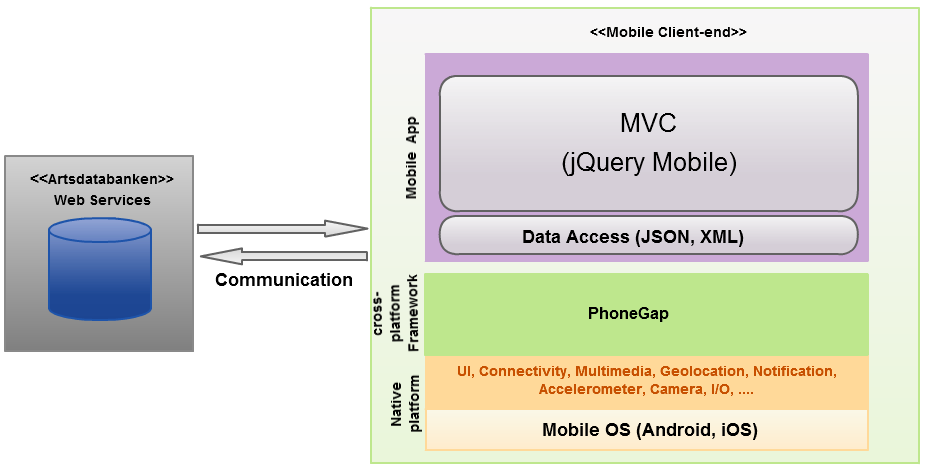
\includegraphics[width=1.0\textwidth]{architecture/architecture.png}
	\caption{Architecture}
	\label{fig:architecture}
\end{figure}

We use a layered architecture, platform-specific issues are avoided using
PhoneGap as a platform-independent layer above the operating system. Following
is a detailed description of each layer, starting at the bottom.

\subsection{Layer 1 - Native operating system}

This layer represents the native operating system for each device (Android, iOs,
blackberry, etc.). Services provided by this layer includes data input/output
operations, geolocation (for some devices), and so on. The operating system is 
our interface to the hardware.

\subsection{Layer 2 - Cross-platform framework}

Layer 1 provides device independent abstractions for file operations, camera
access, geolocation, etc. The primary purpose of this layer is to allow us to
make portable code that can be used on Android, iOs, and other operating systems
with minimal (or no) changes to the code. PhoneGap provides an HTML5,
JavaScript, and CSS interface for the layer above.

\subsection{Layer 3 - Mobile app}

Layer 2 is the actual app, this is where our implementation will be placed.
This layer is split into an internal structure, we use the MVC pattern combined
with some layering. In addition to the componets shown in the diagram, the
jQuery-family of frameworks/utilities is used by model, view and controller.

	\subsubsection{Data access}
	
	The data access sub-layer is responsible for all I/O-operations. This is
	where we access local- and remove storage. The data access layer provides
	domain centric functions for accessing common data sources. E.g.
	ObservationDAO is used to store/retrieve observations to/from local storage.

	\subsubsection{Model}

	The model will be used to represent data used in the app. We can for example
	create a class, Observation, to represent all data related to an
	observation.

	\subsubsection{Controller}

	The controller is responsible coordinating different parts of the system,
	like handling (binding) events.

	\subsubsection{View}

	This component represents the graphical user interface, it entails code for
	generating visual effects, and updating the screen. To save work, we will be
	utilizing functionality (like auto-complete, and common mobile UI
	functionality) from the jQuery-family.
